\section{Empirical Evaluation}

\begin{figure}[t]
\centering
\subfigure{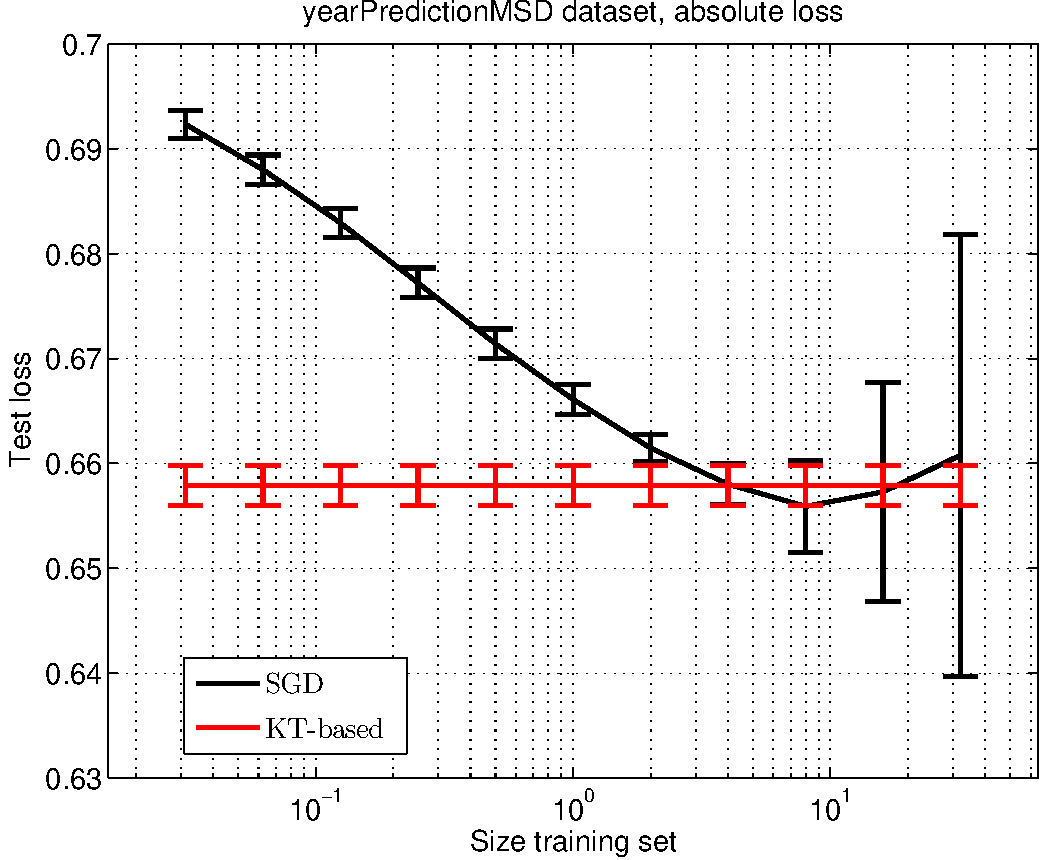
\includegraphics[width=0.32\textwidth]{figs/yearPredictionMSD_kt_train_test-crop.pdf}}
\subfigure{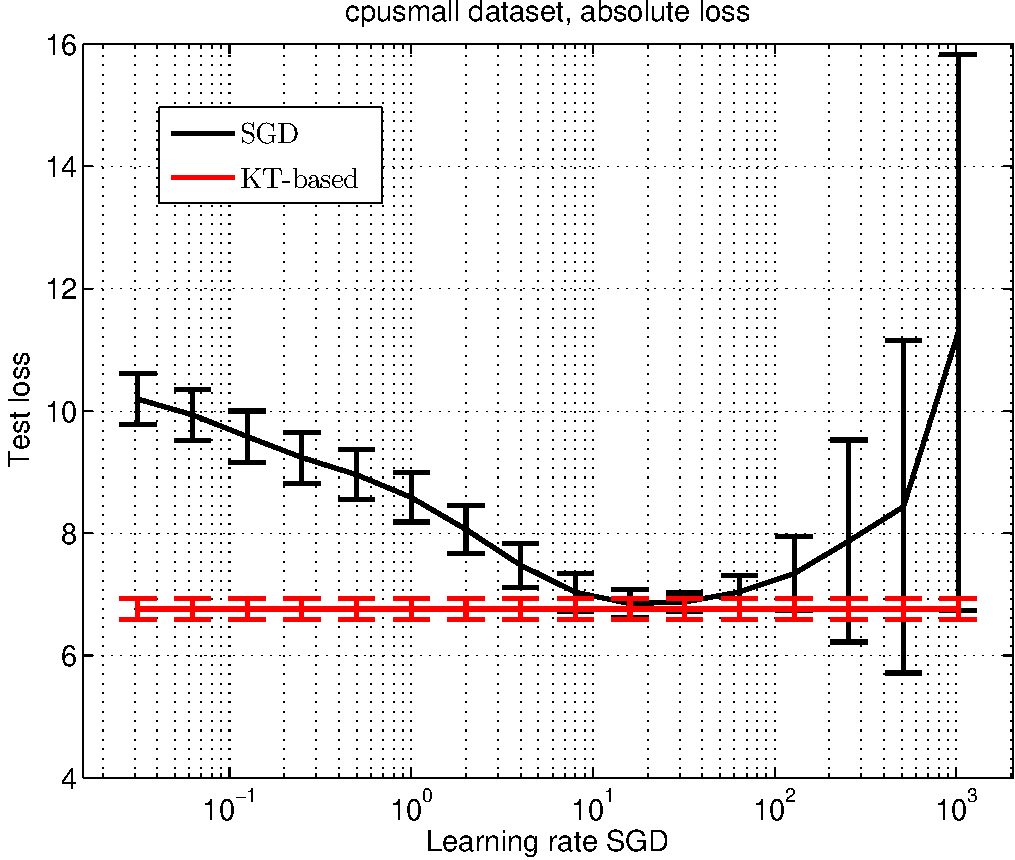
\includegraphics[width=0.32\textwidth]{figs/cpusmall_kt_train_test-crop.pdf}}
\subfigure{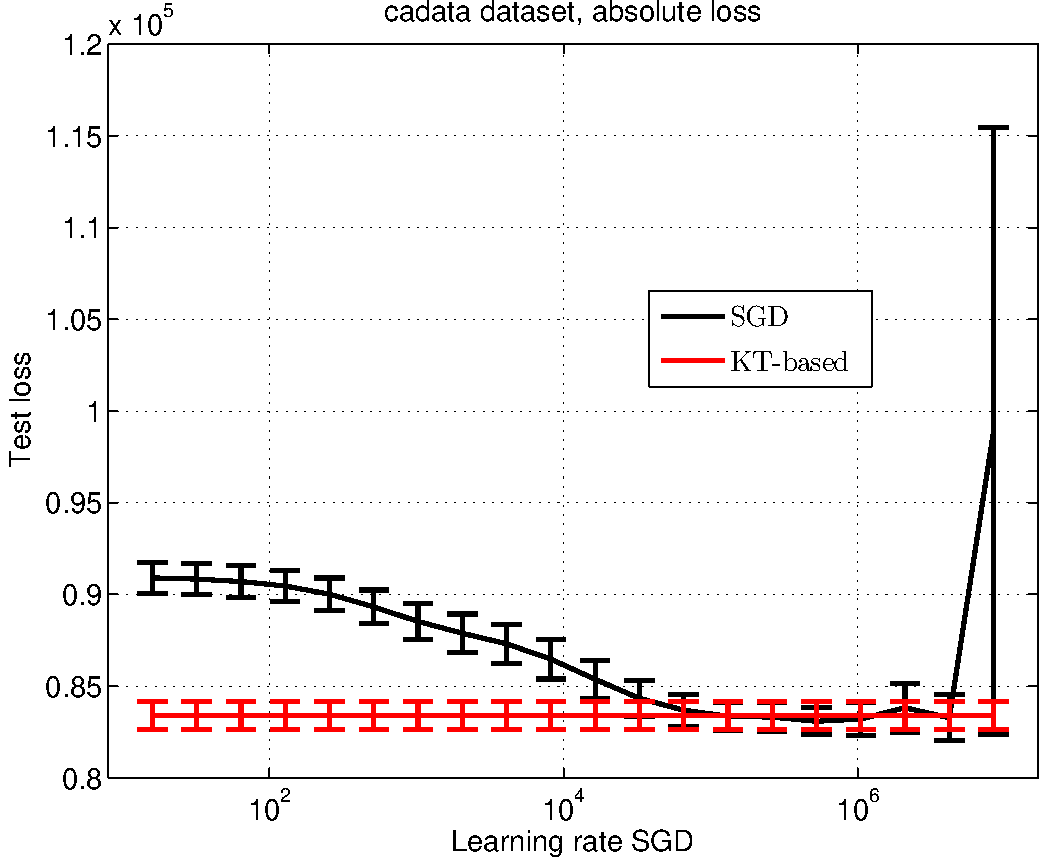
\includegraphics[width=0.32\textwidth]{figs/cadata_kt_train_test-crop.pdf}}
\caption{\footnotesize{Total loss versus learning rate parameter of \ac{SGD} (in log scale), compared with parameter-free algorithms DFEG~\cite{Orabona-2013}, Adaptive Normal~\cite{McMahan-Orabona-2014}, PiSTOL~\cite{Orabona-2014} and Algorithm~\ref{algorithm:kt-sgd}.}}
\label{fig:exp_olo}
\end{figure}

We have run a small empirical evaluation to show that the theoretical difference
between classic learning algorithms and parameter-free ones is real and not just theoretical. In
Figure~\ref{fig:exp_olo}, we have used three regression
datasets\footnote{Datasets available at
\url{https://www.csie.ntu.edu.tw/~cjlin/libsvmtools/datasets/}.}, and solved the
\ac{OCO} problem through \ac{OLO}. In all the three cases, we have used the
absolute loss and normalized the input vectors to have L2 norm equal to 1. From
the empirical results, it is clear that the optimal learning rate is completely
data-dependent, yet \emph{parameter-free algorithms have performance very close
to the unknown optimal tuning of the learning rate}. Moreover, the KT-based
Algorithm~\ref{algorithm:kt-hilbert-space-olo} seems to dominate all the other
similar algorithms.